\documentclass{beamer}
\usetheme{Singapore}
%\usetheme{Copenhagen}
\usecolortheme{seahorse}

\usepackage[utf8]{inputenc}

\usepackage{listings, float, graphicx, lipsum, parallel, verbatim, mathtools, amssymb, hyperref}

\title{ConvLOB}
\subtitle{Stock prices forecasting through CNNs}
\author{Tommaso Battistini \and Edoardo De Matteis}
\date{}

\institute[La Sapienza University of Rome]

\begin{document}

\frame{\titlepage}

\section{Task}

\begin{frame}{Task}
    In today's financial markets most trades are performed electronically and the majority is automated.
    Therefore by analyzing this vast amount of transactions an opportunity has risen.
\end{frame}

\begin{frame}
    Develop a deep neural network that leverages the attention mechanism to predict future stock price movements in the F1-2010 high-frequency LOB Dataset.
\end{frame}

\section{LOB}
\begin{frame}{Limit Order Book (LOB)}
    The Limit Order Book (LOB) has three components: \textbf{buy orders}, \textbf{sell orders} and \textbf{order history}.
    These are organized in \textbf{price levels}.

    Buy/sell (ask/bid) limit orders will sit in the order book until an order of the opposite type matches their price
\end{frame}

\begin{frame}
    Both \textbf{bid} and \textbf{ask} orders are characterized by a price and volume.

    \begin{equation}
        (p_a, v_a, p_b, v_b)
    \end{equation}

    The distance between the highest bid order and the lowest ask order is called \textbf{spread}, the average betweem them is also called \textbf{mid price}.
\end{frame}

\begin{frame}
    \centering
    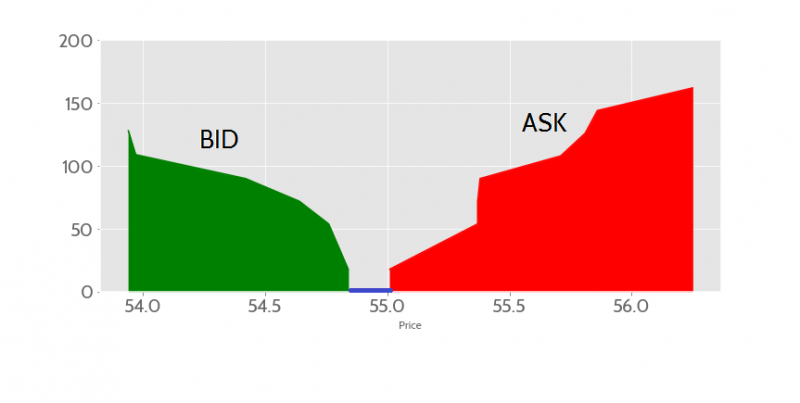
\includegraphics[scale=0.38]{imgs/asf.png}
\end{frame}

\section{Data}
\begin{frame}{Dataset}
    We used the \textit{F1-2010} dataset in order to train and test our model.
    Its data consist of high-frequency limit order data extracted from the \textit{Nasdaq Nordic} stock market, for a window of 10 consecutive days.
\end{frame}

\begin{frame}
    We have a total of 40 features for each timestamp, since each state of the LOB contains 10 levels of both buy and sell orders.

    Data have been used as follows:
    \begin{itemize}
        \item We used 5 days for training.
        \item 2 days were used for validation i.e. we have a 80/20 split.
        \item Last 3 days for testing.
    \end{itemize}
\end{frame}

\begin{frame}{Normalization}
    In order to obtain the best possible performances, data are already normalized using $z$-score normalization:
    \begin{equation}
        z = \frac{x - \mu}{\sigma}
    \end{equation}
\end{frame}

\begin{frame}{Labelling}
    In order to create labels that somehow represent the direction of changes in price, we use the mid price:

    \begin{equation}
        p_t = \frac{p_a + p_b}{2}
    \end{equation}

    We may use \textbf{strict} or \textbf{smooth} labelling, in F1-2010 the latter is applied by default.

    Labels are computed using the mean of $k$ steps' mid-prices, comparing the percentage change against a threshold $\alpha$:
\end{frame}

\begin{frame}{Smooth labelling}
    \begin{align}
        m_t & = \frac{1}{k} \sum_{i=0}^k p_{t+1}     \\
        l_t & = \frac{m_t - p_t}{p_t}                \\
        l_t & > \alpha \Rightarrow \quad \uparrow    \\
        l_t & = \alpha \Rightarrow \quad \rightarrow \\
        l_t & < \alpha \Rightarrow \quad \downarrow
    \end{align}
\end{frame}

\section{Model}
\begin{frame}{Model Architecture}
    Our models' architectures revolve around 3 main layers:
    \begin{itemize}
        \item Convolutional modules.
        \item Multi-head attention modules.
        \item Classification heads.
    \end{itemize}
\end{frame}

\begin{frame}{Convolutional model}
    This model is inspired by reference paper's model, we exploit 2D temporal convolution, thus we need to reshape input data to a compatible shape.
    \begin{equation*}
        100, 40 \longrightarrow 100, 40, 1
    \end{equation*}
\end{frame}

\begin{frame}
    \begin{figure}
        \centering
        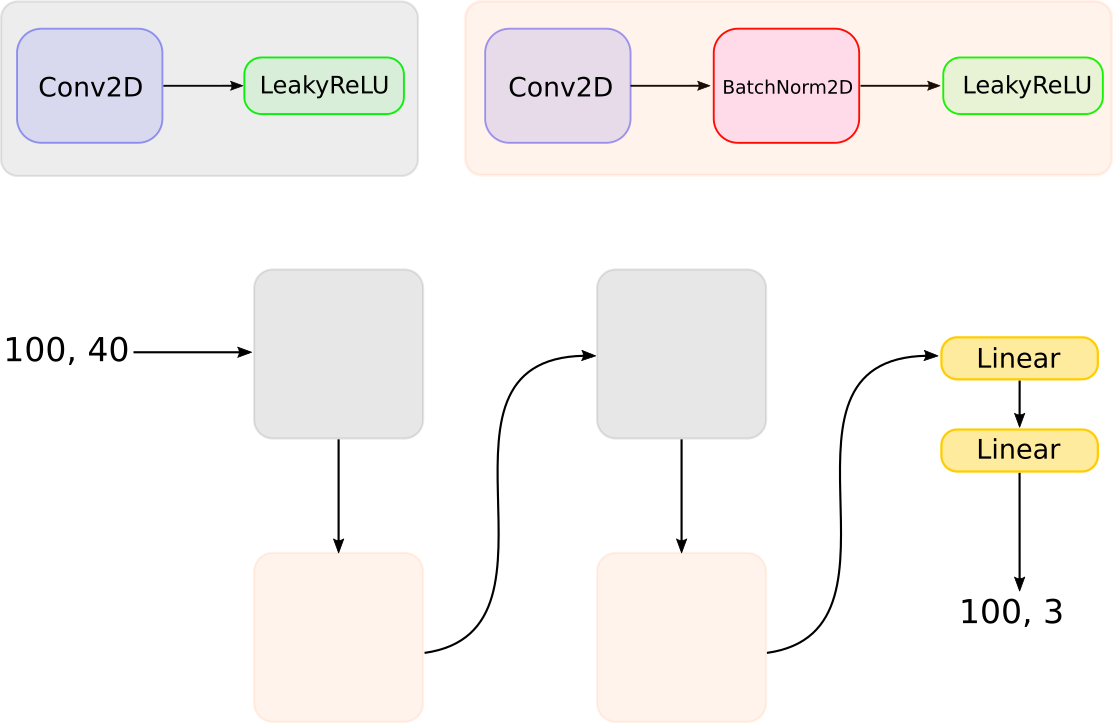
\includegraphics[scale=0.35]{imgs/conv.png}
    \end{figure}
\end{frame}

\begin{frame}{Attention model}
    Again we use 2D temporal convolutions, yet data is reshaped in a more channel-centered model.
    \begin{equation*}
        100, 40 \longrightarrow 100, 10, 4
    \end{equation*}
    Furtherly to learn sequential data we introduce a multi-head attention module.
\end{frame}

\begin{frame}
    \begin{figure}
        \centering
        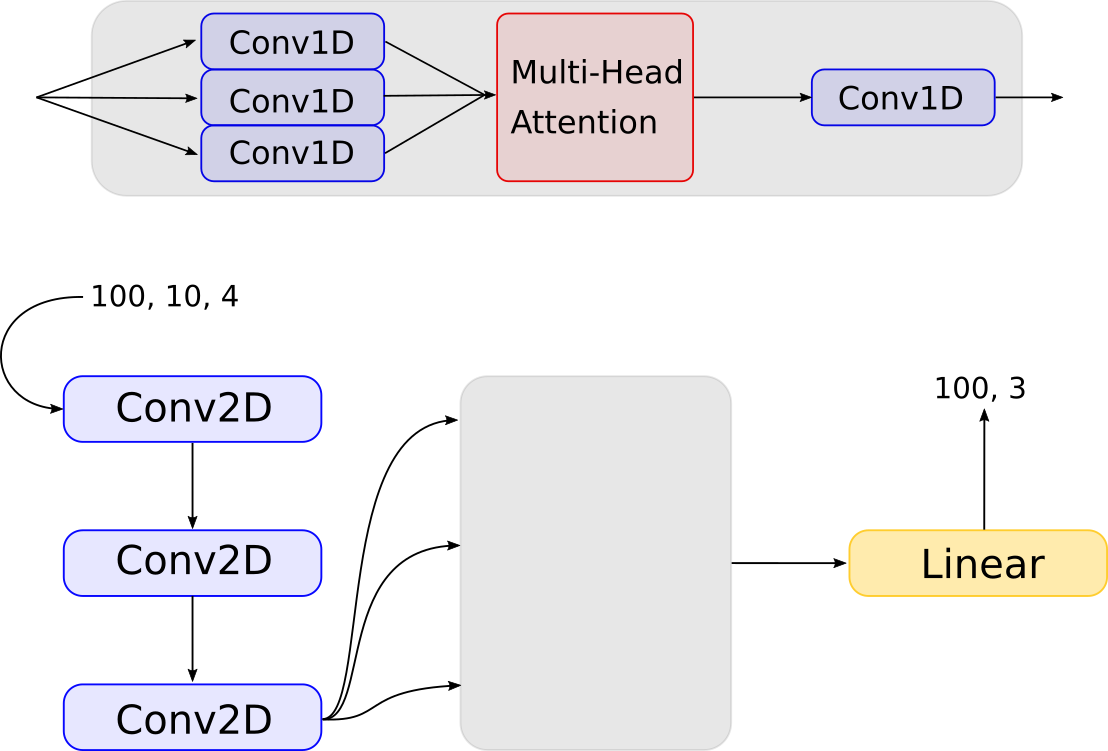
\includegraphics[scale=0.35]{imgs/attention.png}
    \end{figure}
\end{frame}

\section{Experiments}
\begin{frame}{Convolutional model}
    \begin{center}
        \begin{tabular}{ l l l l l }
                               & \textbf{Epoch} & \textbf{LR} & \textbf{F1} & \textbf{Cohen K} \\
            \hline
            Tsantedekis et. al & -              & -           & 55.21       & 0.35             \\
            CNN                & 36             & 0.001       & \textbf{60} & 0.36             \\
            Att                & 99             & 0.001       & 59.2        & \textbf{0.38}    \\
            \hline
        \end{tabular}
    \end{center}
\end{frame}

\begin{frame}
    \centering
    \huge{\textit{Thank You.}}
\end{frame}

\end{document}